\documentclass{article}

% \usepackage{standalone}
 \usepackage{graphicx}
% \usepackage{media9}
%\graphicspath{{./images/}}
% \usepackage{amsmath}
\usepackage{multicol}
\usepackage{hyperref}
% \usepackage{setspace}                       \usepackage{geometry}          
%  \usepackage{longtable}                      
% \usepackage{chicago}                  
% \usepackage{times} 
% \usepackage{paracol}   % parallel columns    
% \usepackage[dvipsnames]{xcolor}       \usepackage{calc}                                      

% \usepackage{tikz}
% \usetikzlibrary{positioning, shadows, arrows, automata, shapes, calc, decorations.pathreplacing,calligraphy}

\title{Notes on Experiments}
\begin{document}
\maketitle
\tableofcontents \newpage
BASELINE PARAMETERS
\begin{verbatim}

        # LABOUR MARKET AND FIRM PARAMETERS
            'subsistence_wage': 40000., # psi
            'init_city_extent': 10.,    # CUT OR CHANGE?
            'seed_population': 400,
            'init_wage_premium_ratio': 0.2, # 1.2, ###

            # PARAMETERS MOST LIKELY TO AFFECT SCALE
            'c': 300                             ### .0,                            ###
            'price_of_output': 10,                 ######
            'density':600,                         #####
            'A': 3000,
            'alpha': 0.18,
            'beta':  0.75,
            'gamma': 0.12, ### reduced from .14
            'overhead': 1.5,
            'mult': 1.2,
            'adjN': 0.15,
            'adjk': 0.10,
            'adjn': 0.15,
            'adjF': 0.02,
            'adjw': 0.05, 
            'dist': 1, 
            'init_F': 100.0,
            'init_k': 500.0,
            'init_n': 100.0,

            # HOUSING AND MORTGAGE MARKET PARAMETERS
            'mortgage_period': 5.0,       # T, in years
            'working_periods': 40,        # in years
            'savings_rate': 0.3,
            'discount_rate': 0.07,        # 1/delta    Check THIS
            'r_prime': 0.05,
            'r_margin': 0.01,
            'property_tax_rate': 0.04,     # tau, annual rate, was c
            'housing_services_share': 0.3, # a
            'maintenance_share': 0.2,      # b
            'max_mortgage_share': 0.9,
            'ability_to_carry_mortgage': 0.28,
            'wealth_sensitivity': 0.1,
            'capital_gains_tax_person':   0.0, # share 0-1
            'capital_gains_tax_investor': 1, # share 0-1
    
\end{verbatim}
\newpage

% \section{parameters}
% \begin{verbatim}

% \end{verbatim}
 \section{Change Density}
 This experiment verifies that the labour-market/urban model that is the platform for the housing market analysis behaves exactly as expected when density changes. mpl, n,N,F,E and k all rise.
 
\begin{tabular}{|c|c||c|c||c|c|}
mpl  & up & n   &  up & N   &  up \\
F    & up   & E   &  up  &  k & up
\end{tabular} 

 \hspace*{-2cm}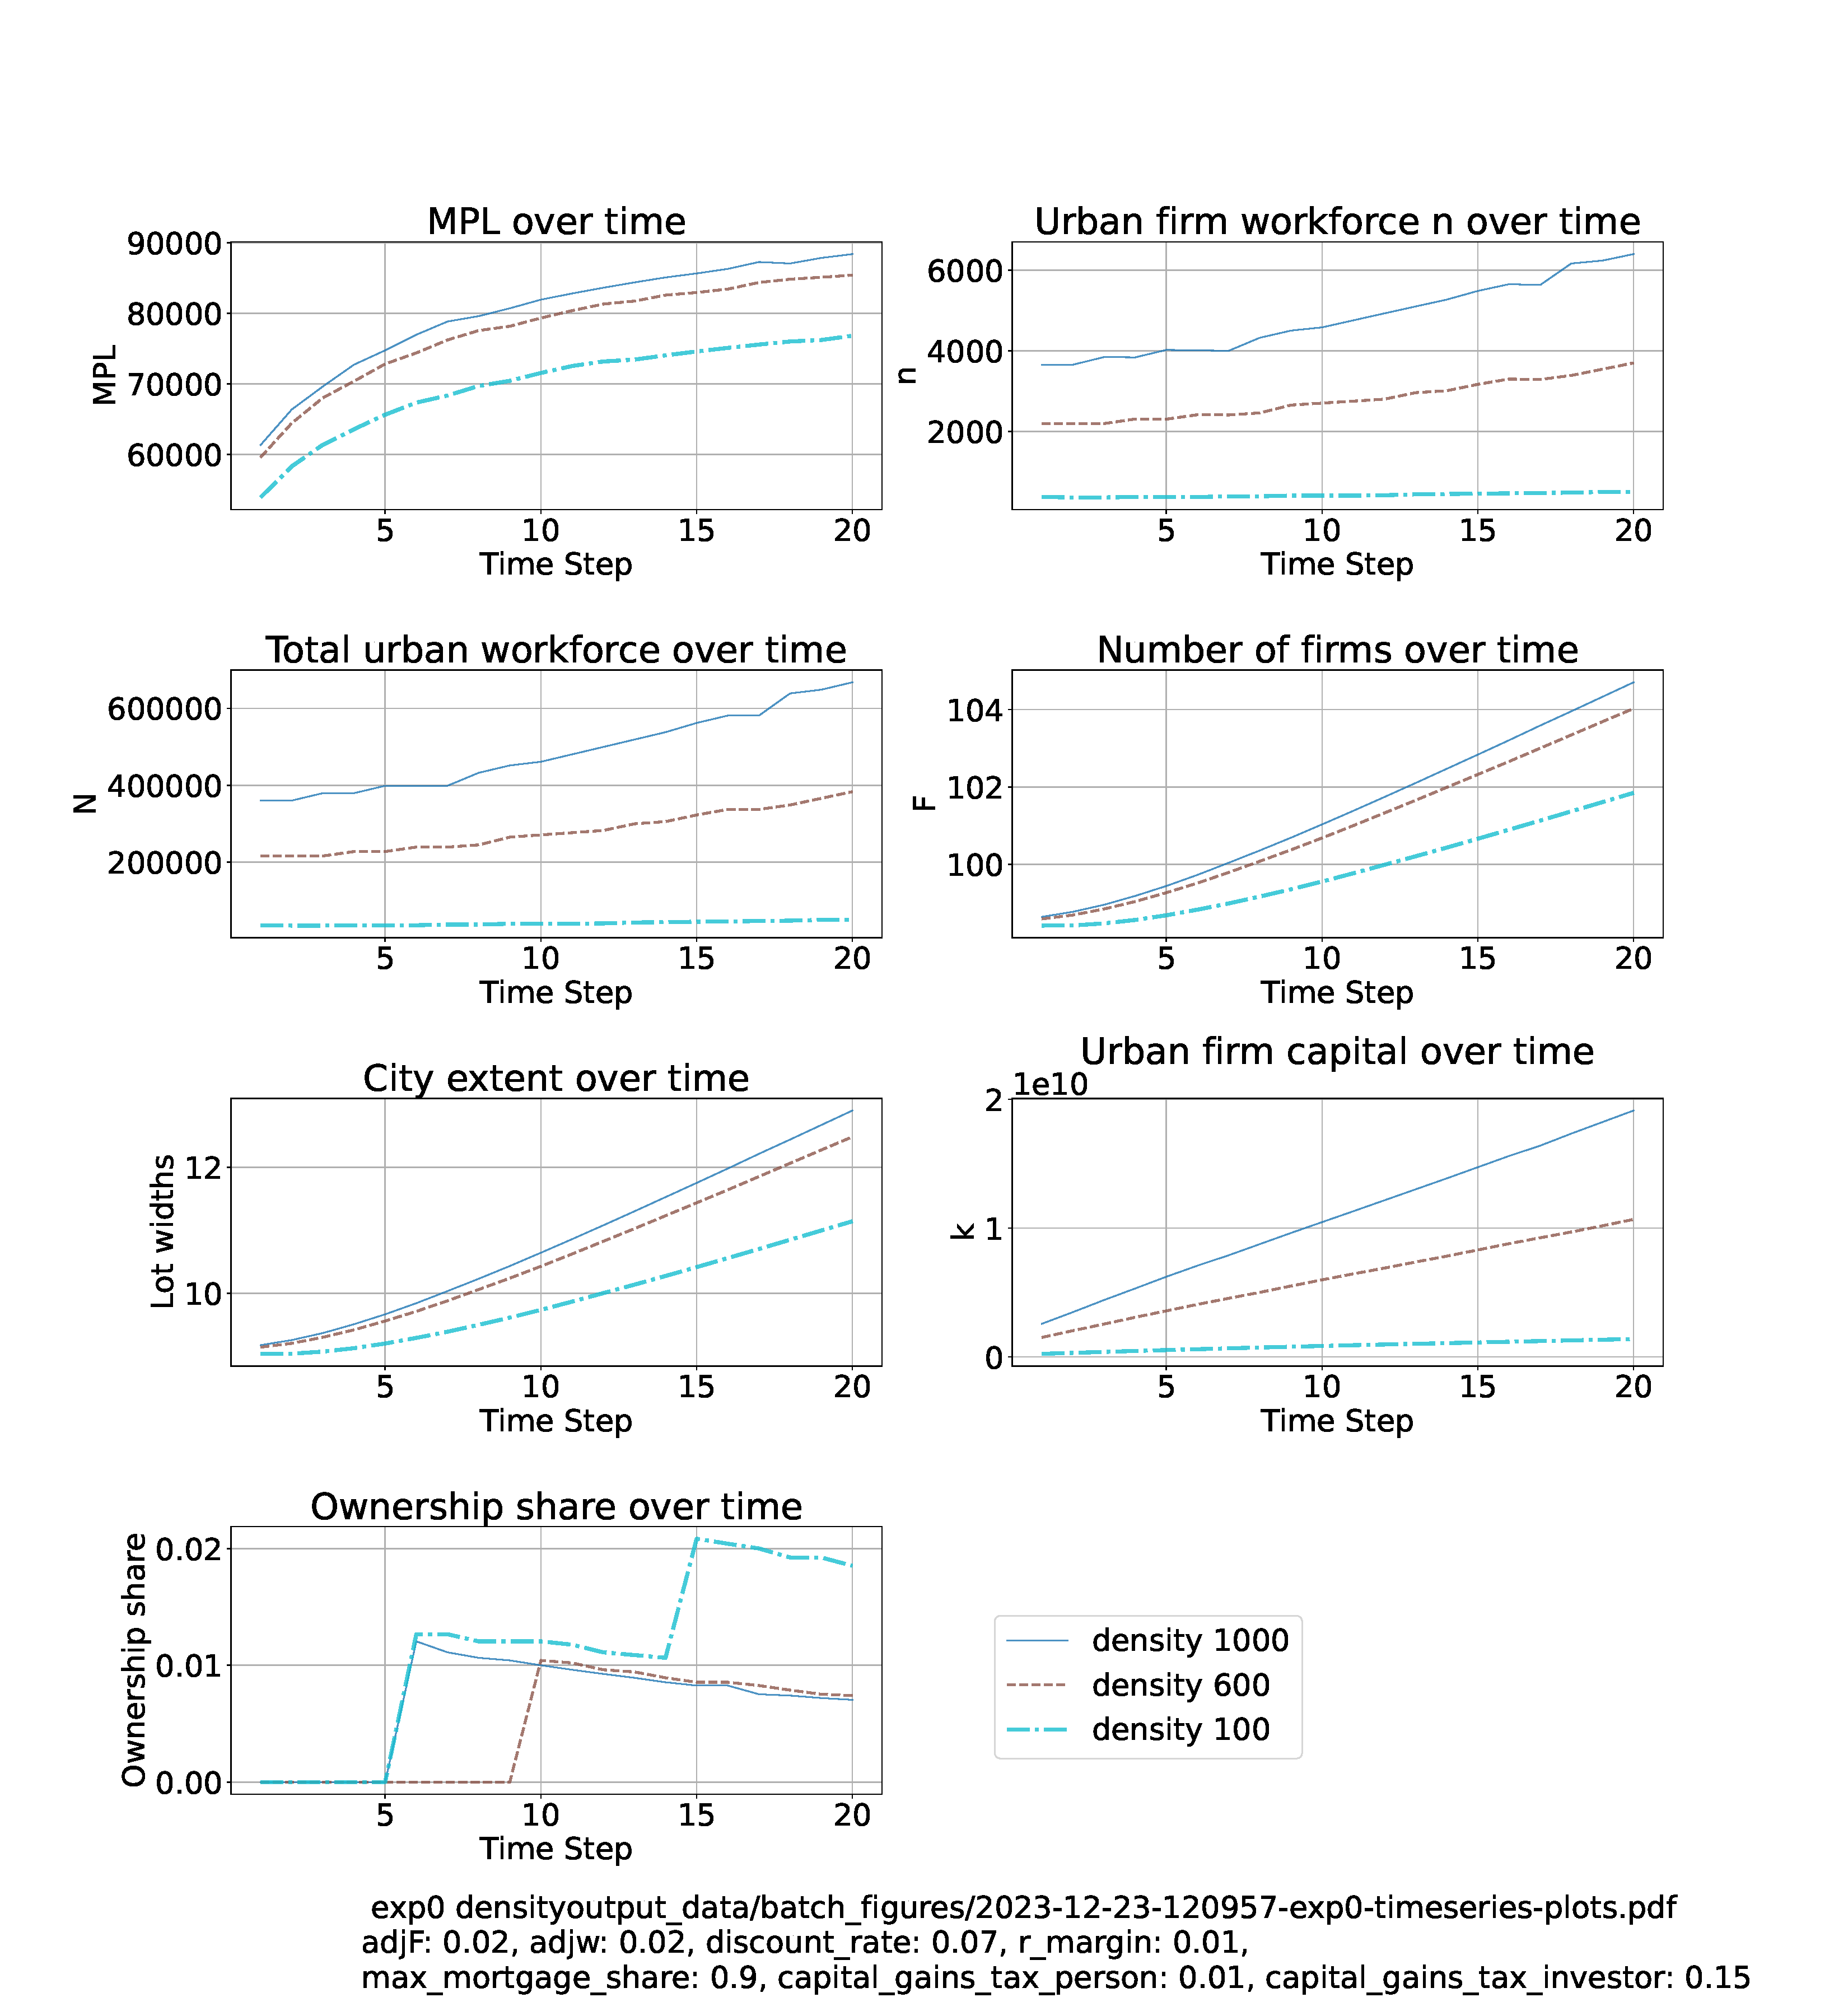
\includegraphics[trim= 1.5cm 3.65cm 2cm 4.0cm, clip, scale=.3]{Density-3-20.pdf}

\newpage %%%%%%%%%%%%%%%%%%%%%%%%%%%%%%%%%%

\section{High Gamma}
Very high levels of the agglomeration parameter Gamma are implausible. They drive up marginal productivity, causing very rapid growth, drive down firm size because the first worker is extremely productive but the MPL falls rapidly. Very small firms with high levels of capital multiply. Rapidly rising prices encourage investors while savings-limited owner-occupiers are squeezed out.
 
\begin{tabular}{|c|c||c|c||c|c|}
mpl  & up   & n   & up & N   &  up \\
F    & up   & E   &  up  &  k & up
\end{tabular} 

 \hspace*{-2.5cm}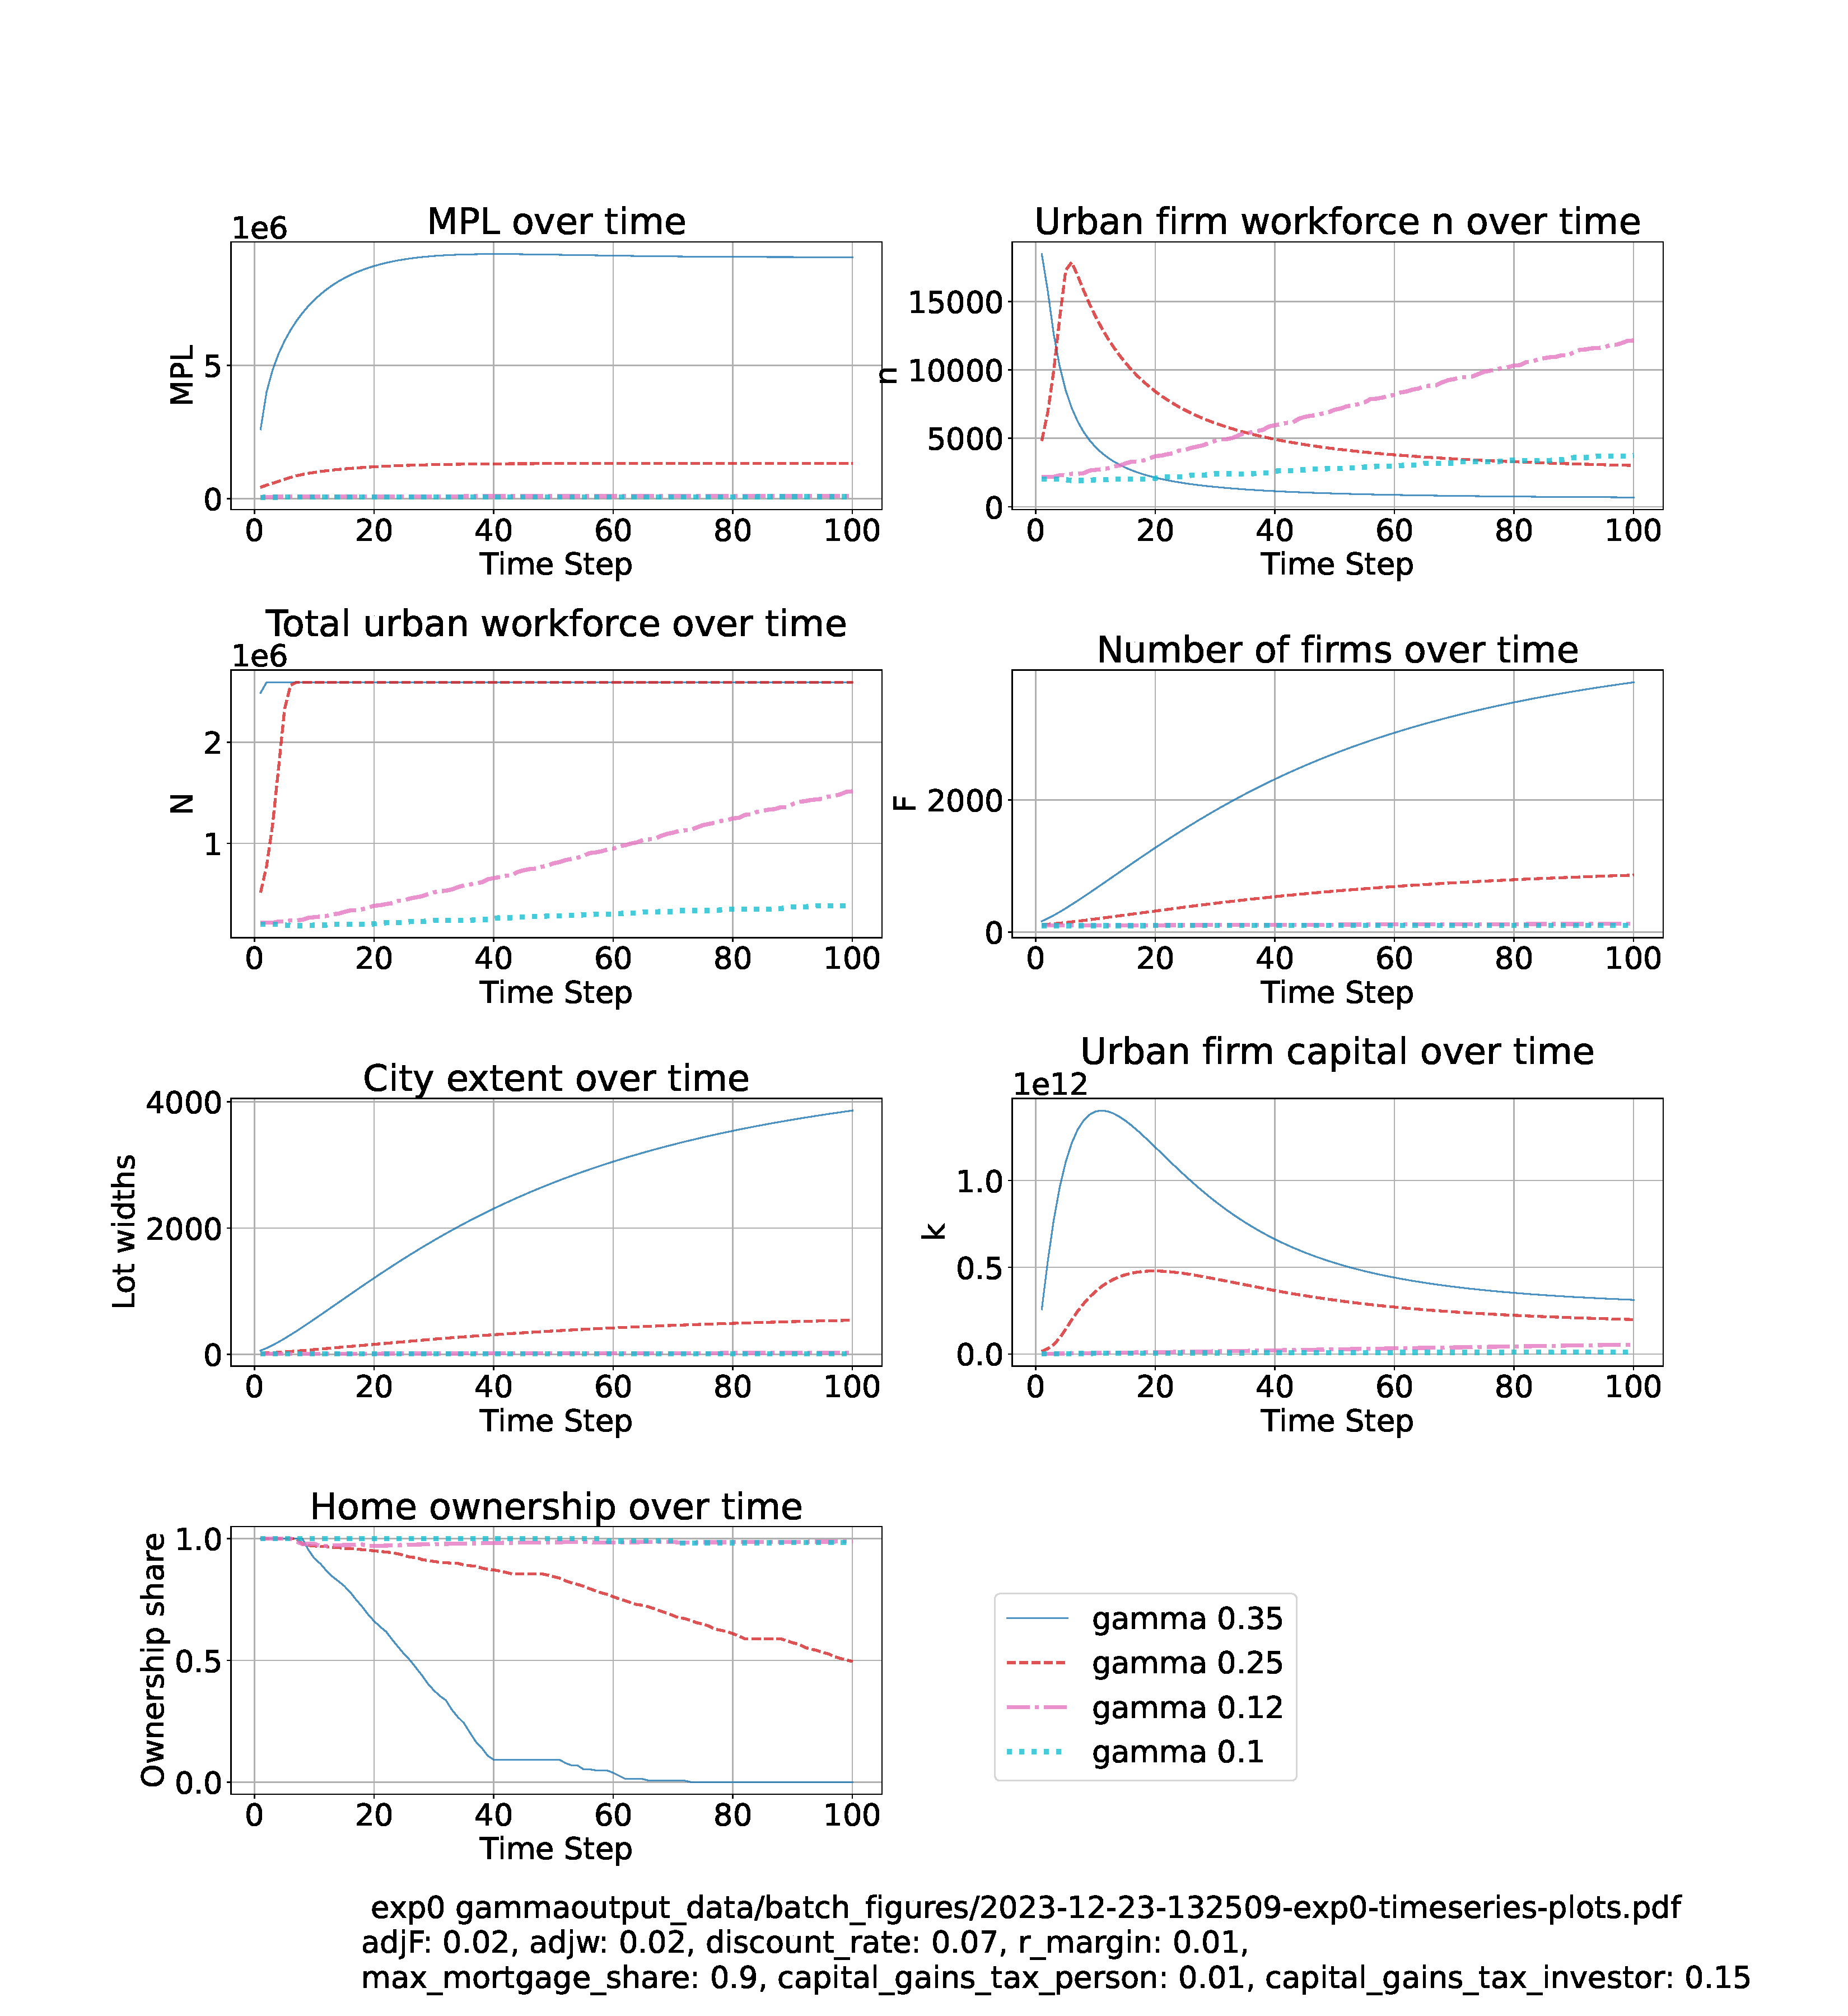
\includegraphics[trim= 1.5cm 3.65cm 2cm 4.0cm, clip, scale=.28]{fig/Analysis/Gamma-5-30.pdf}

\newpage %%%%%%%%%%%%%%%%%%%%%%%%%%%%%%%%%%
\section{Low Gamma}
Low levels of the agglomeration parameter Gamma are plausible but city growth requires a level high enough to overcome decreasing returns in production.
 
\begin{tabular}{|c|c||c|c||c|c|}
mpl  & up   & n   & up & N   &  up \\
F    & up   & E   &  up  &  k & up
\end{tabular} 

 \hspace*{-2.5cm}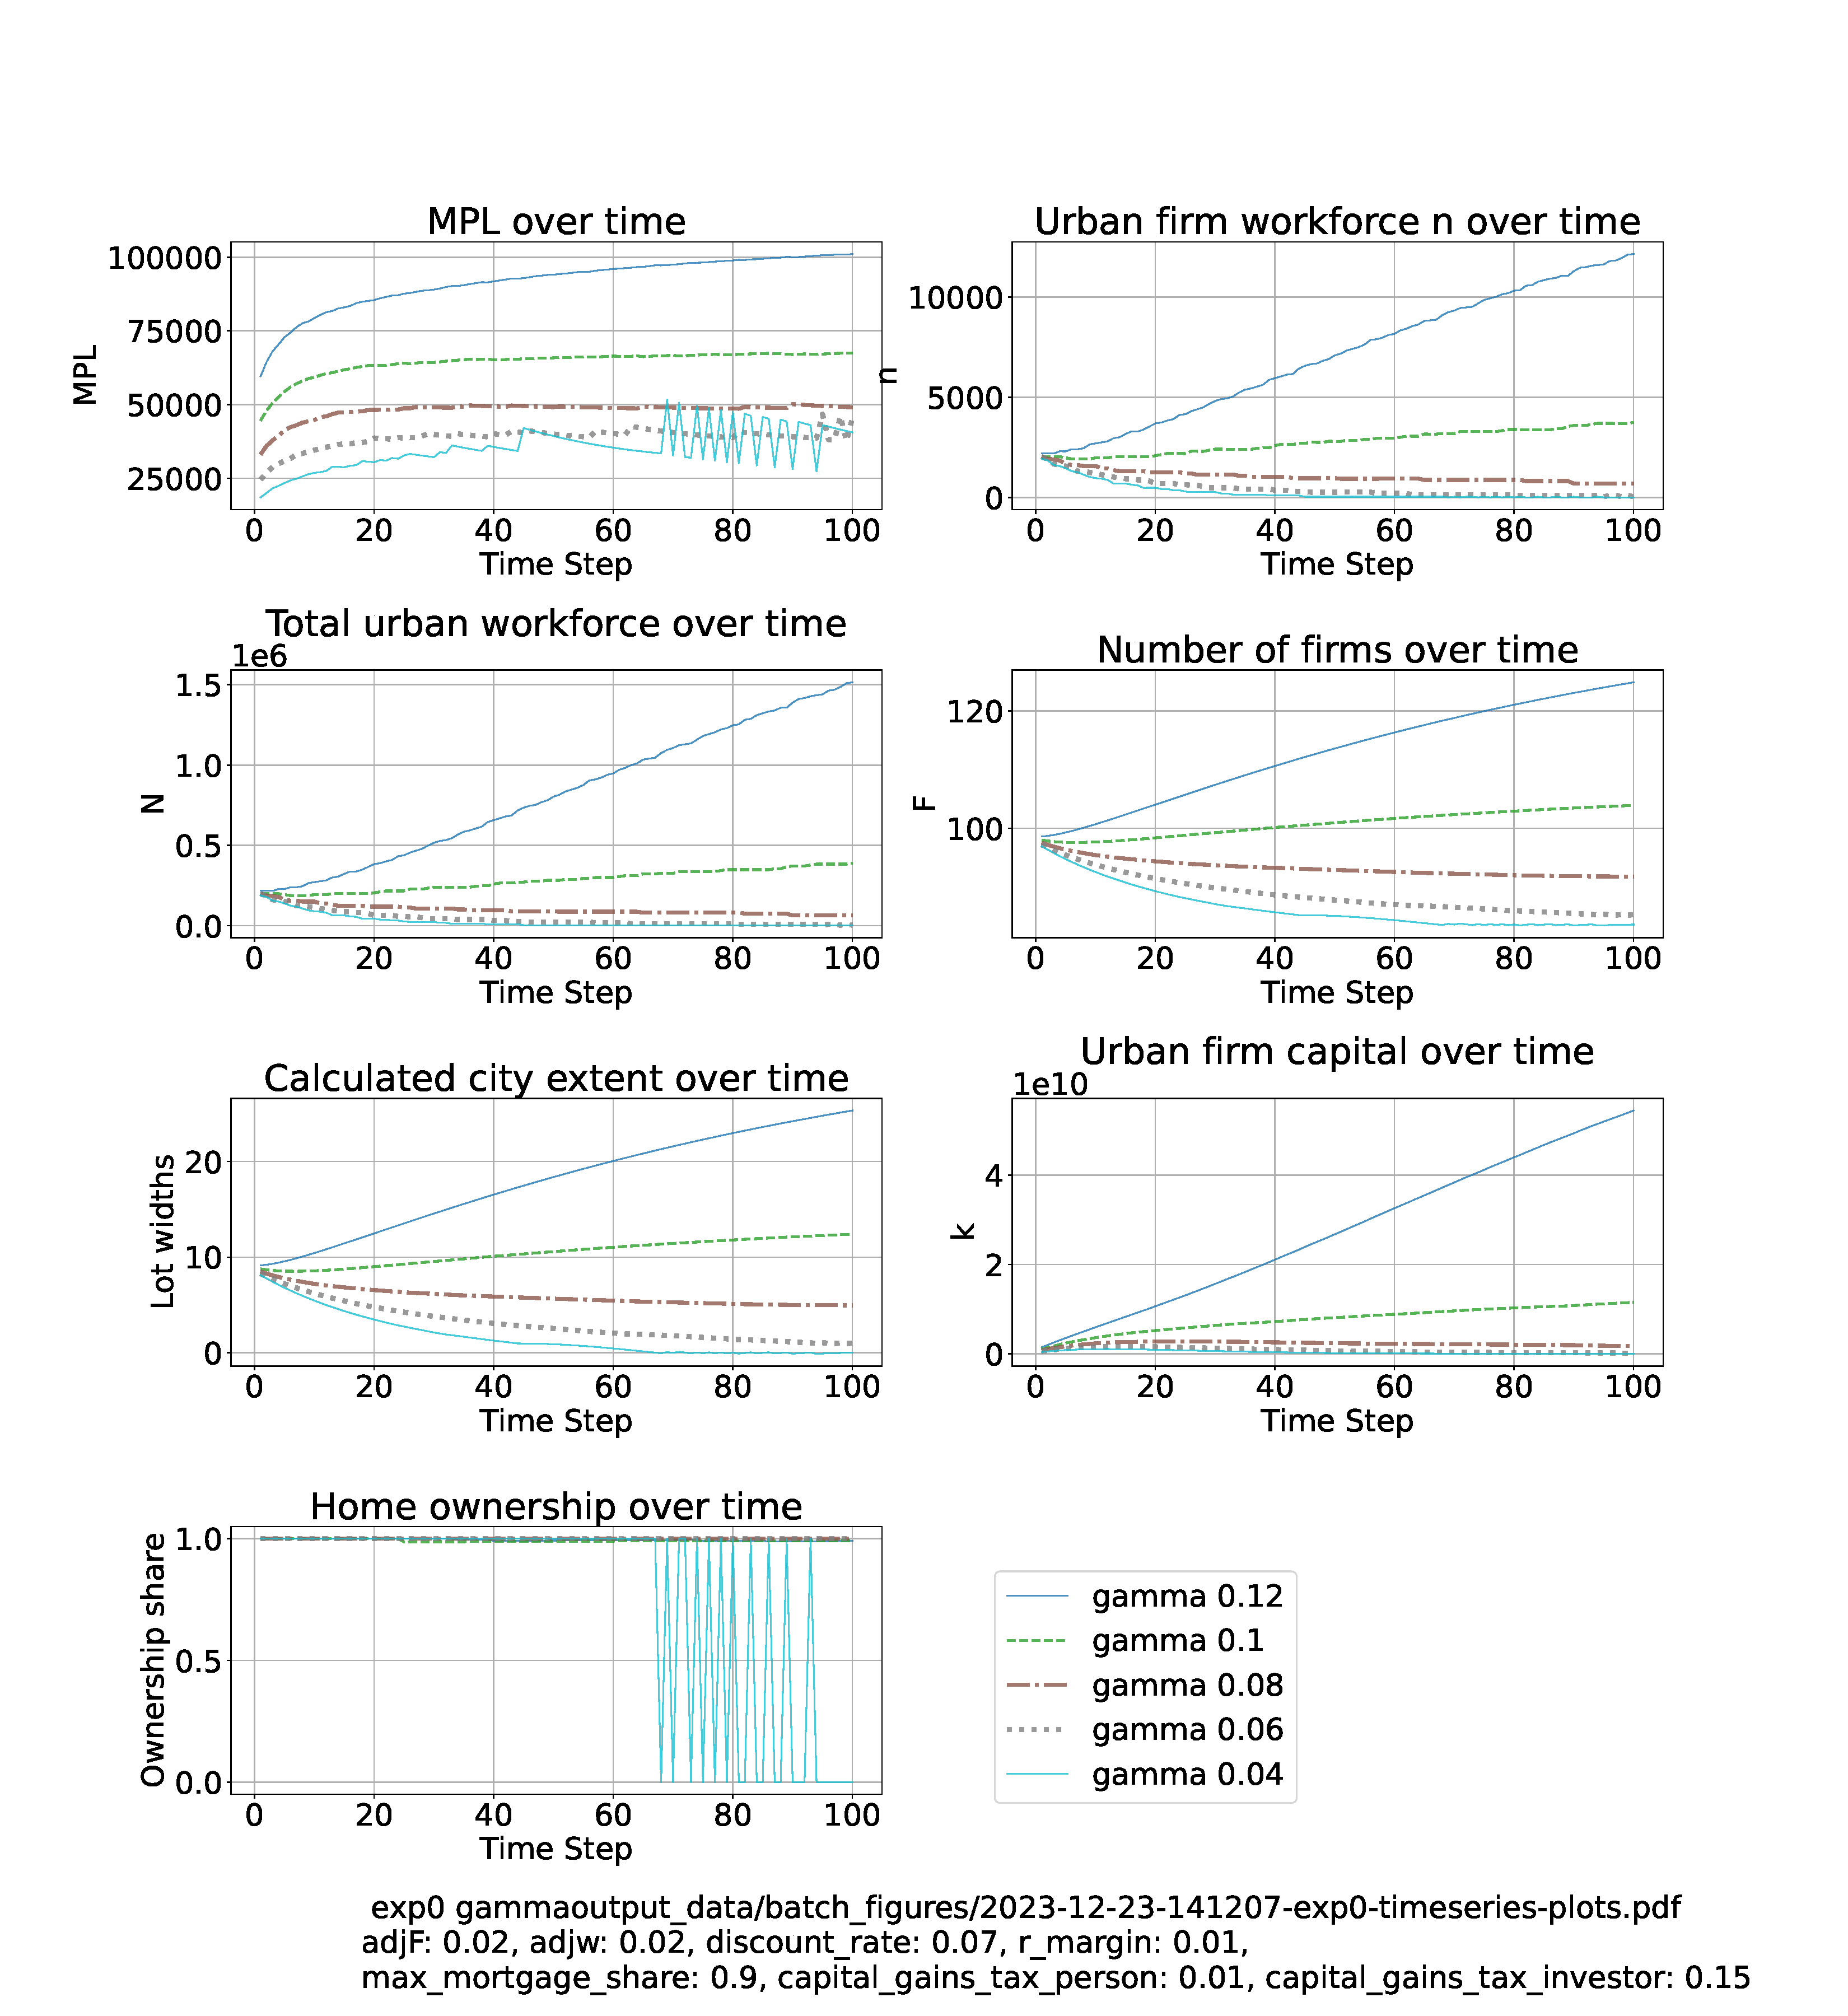
\includegraphics[trim= 1.5cm 3.65cm 2cm 4.0cm, clip, scale=.3]{fig/Analysis/Gamma-low-5-30.pdf}

\newpage %%%%%%%%%%%%%%%%%%%%%%%%%%%%%%%%%%



\newpage %%%%%%%%%%%%%%%%%%%%%%%%%%%%%%%%%%

\section{Alpha}
Low levels of capital productivity lead to urban decline. City growth requires a level high enough to overcome decreasing returns in production. Capital augmenting public expenditures would support growth.
 
\begin{tabular}{|c|c||c|c||c|c|}
mpl  & up   & n   & \textbf{down} & N   &  up \\
F    & up   & E   &  up  &  k & up
\end{tabular} 

 \hspace*{-2.5cm}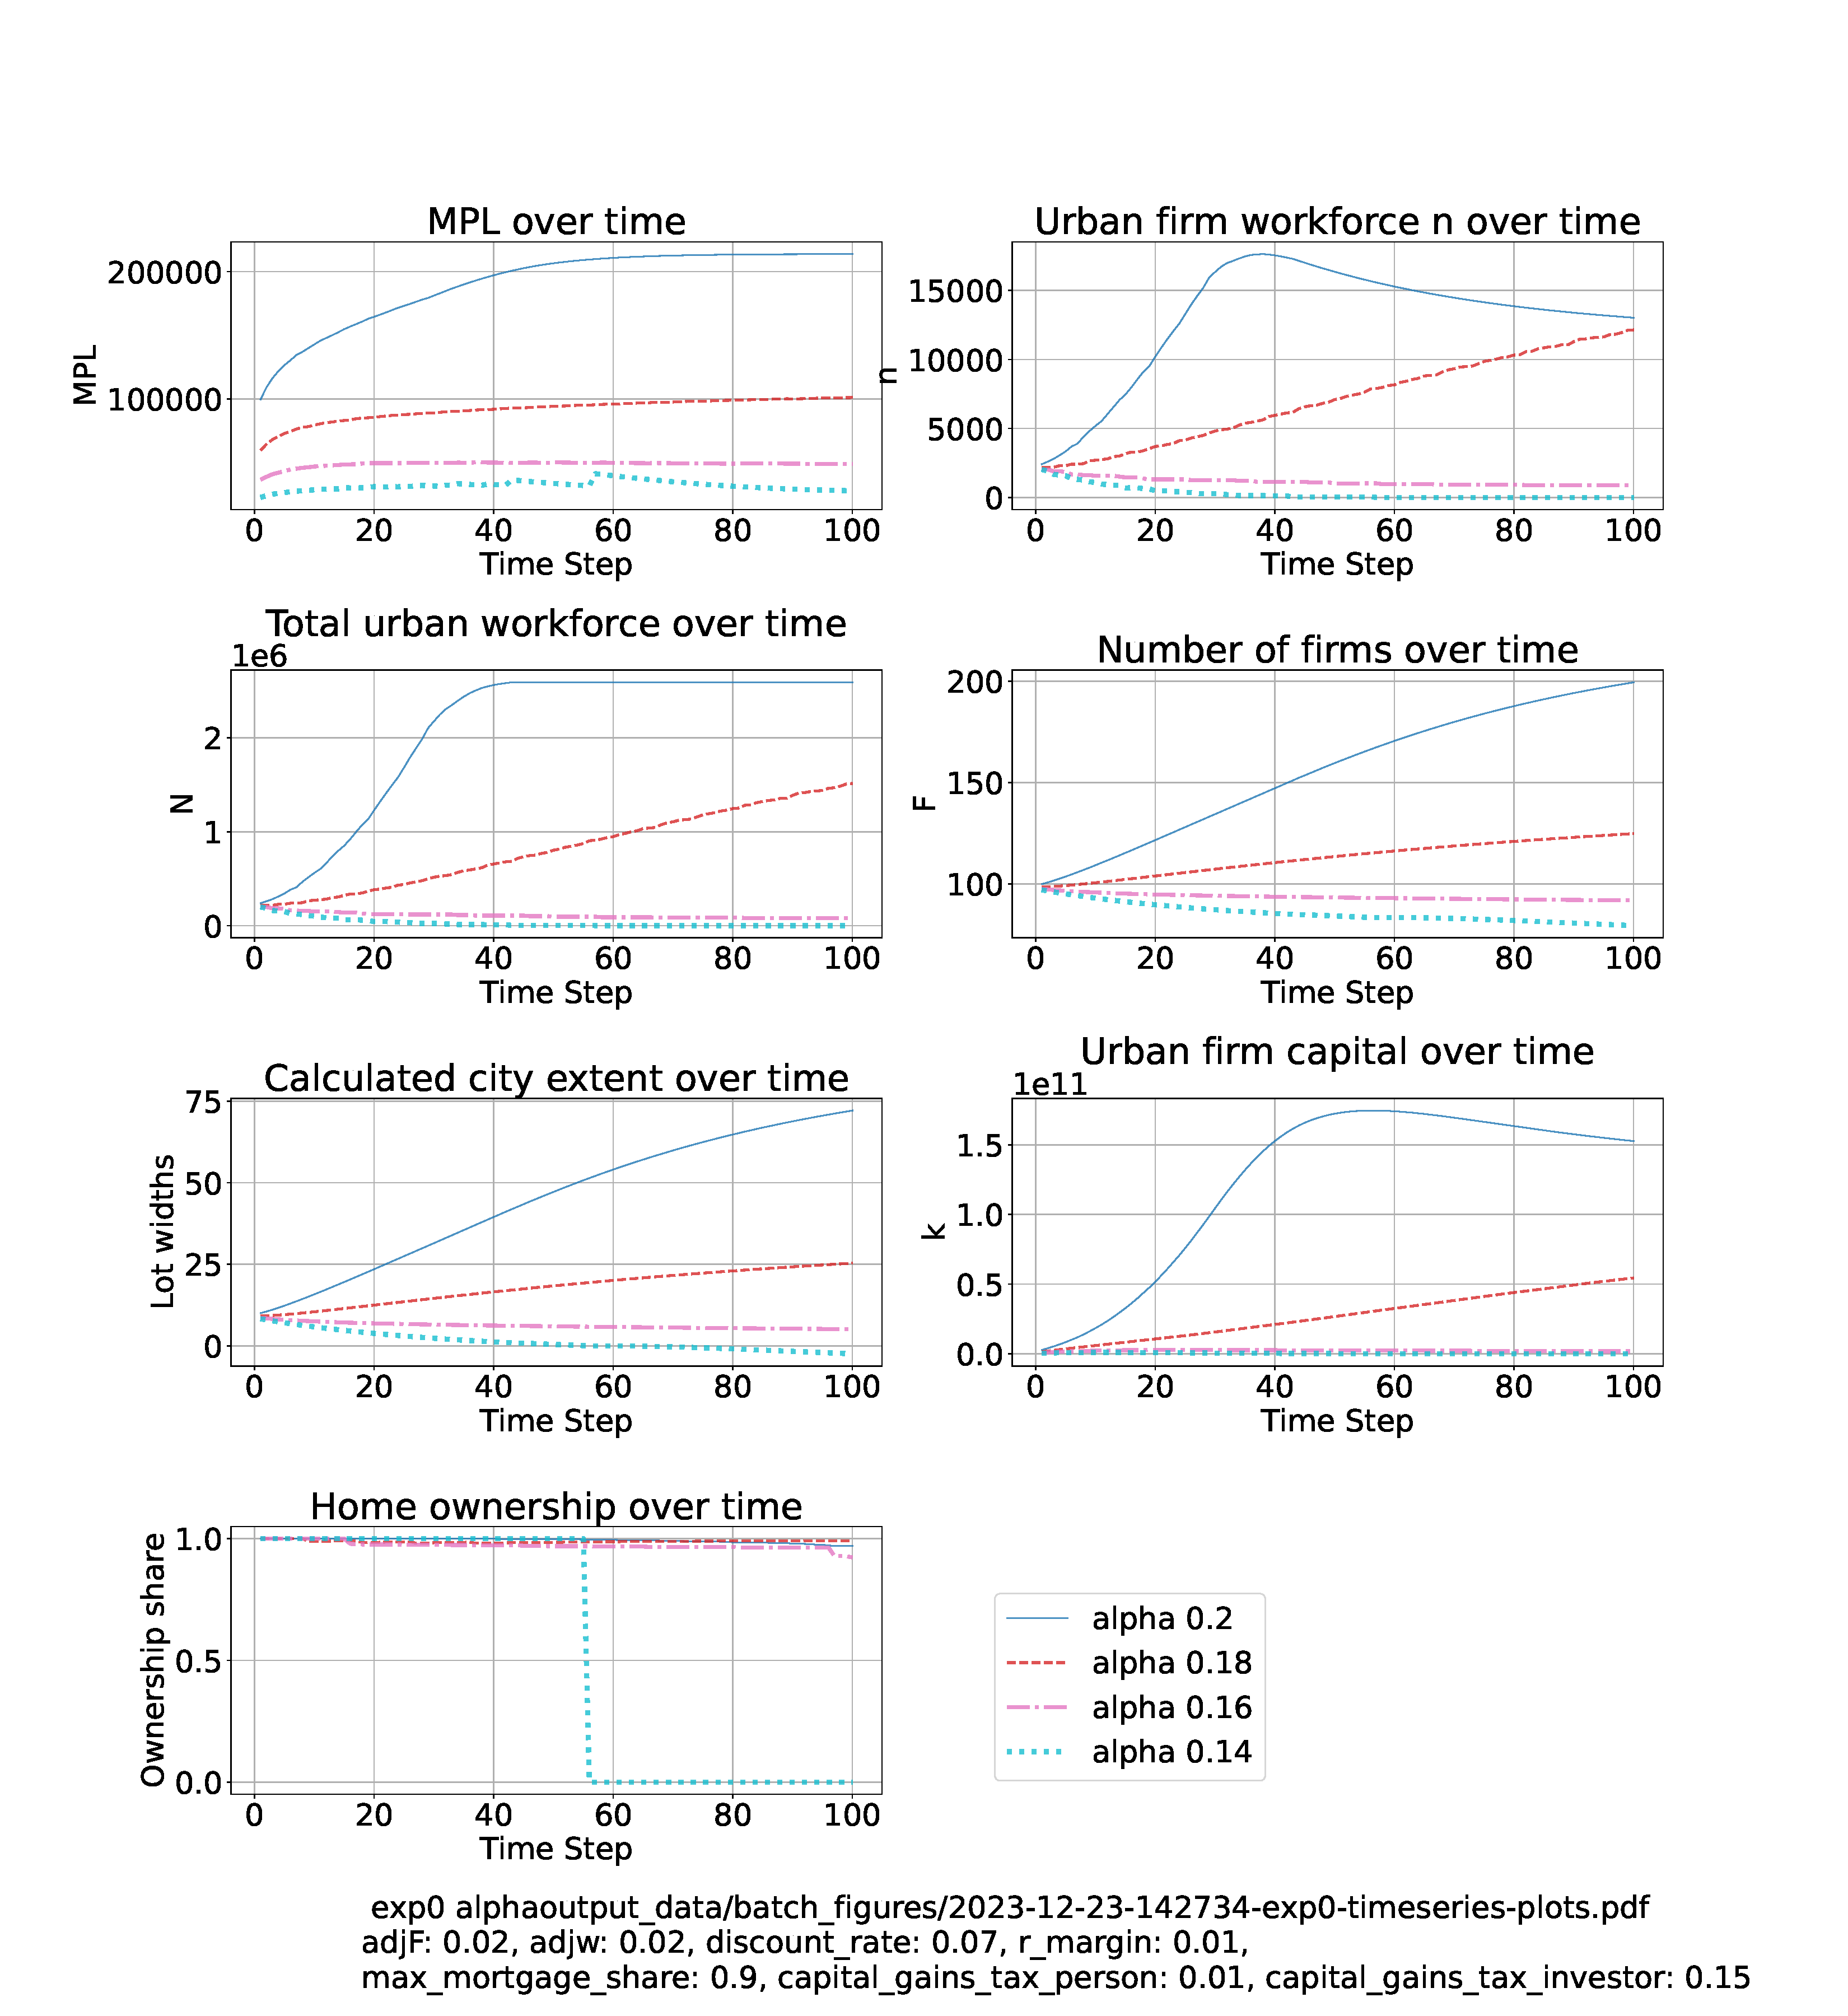
\includegraphics[trim= 1.5cm 3.65cm 2cm 4.0cm, clip, scale=.3]{fig/Analysis/Alpha-4-30.pdf}

\newpage %%%%%%%%%%%%%%%%%%%%%%%%%%%%%%%%%%

\section{Transportation cost c}
Transport cost affects the city extent, in turn affecting workforce size and the wealth generated on the city's land. All variables respond as expected. 
 
\begin{tabular}{|c|c||c|c||c|c|}
mpl  & null   & n   & null & N   &  null \\
F    & null   & E   &  null  &  k & null
\end{tabular} 

 \hspace{-2.5cm}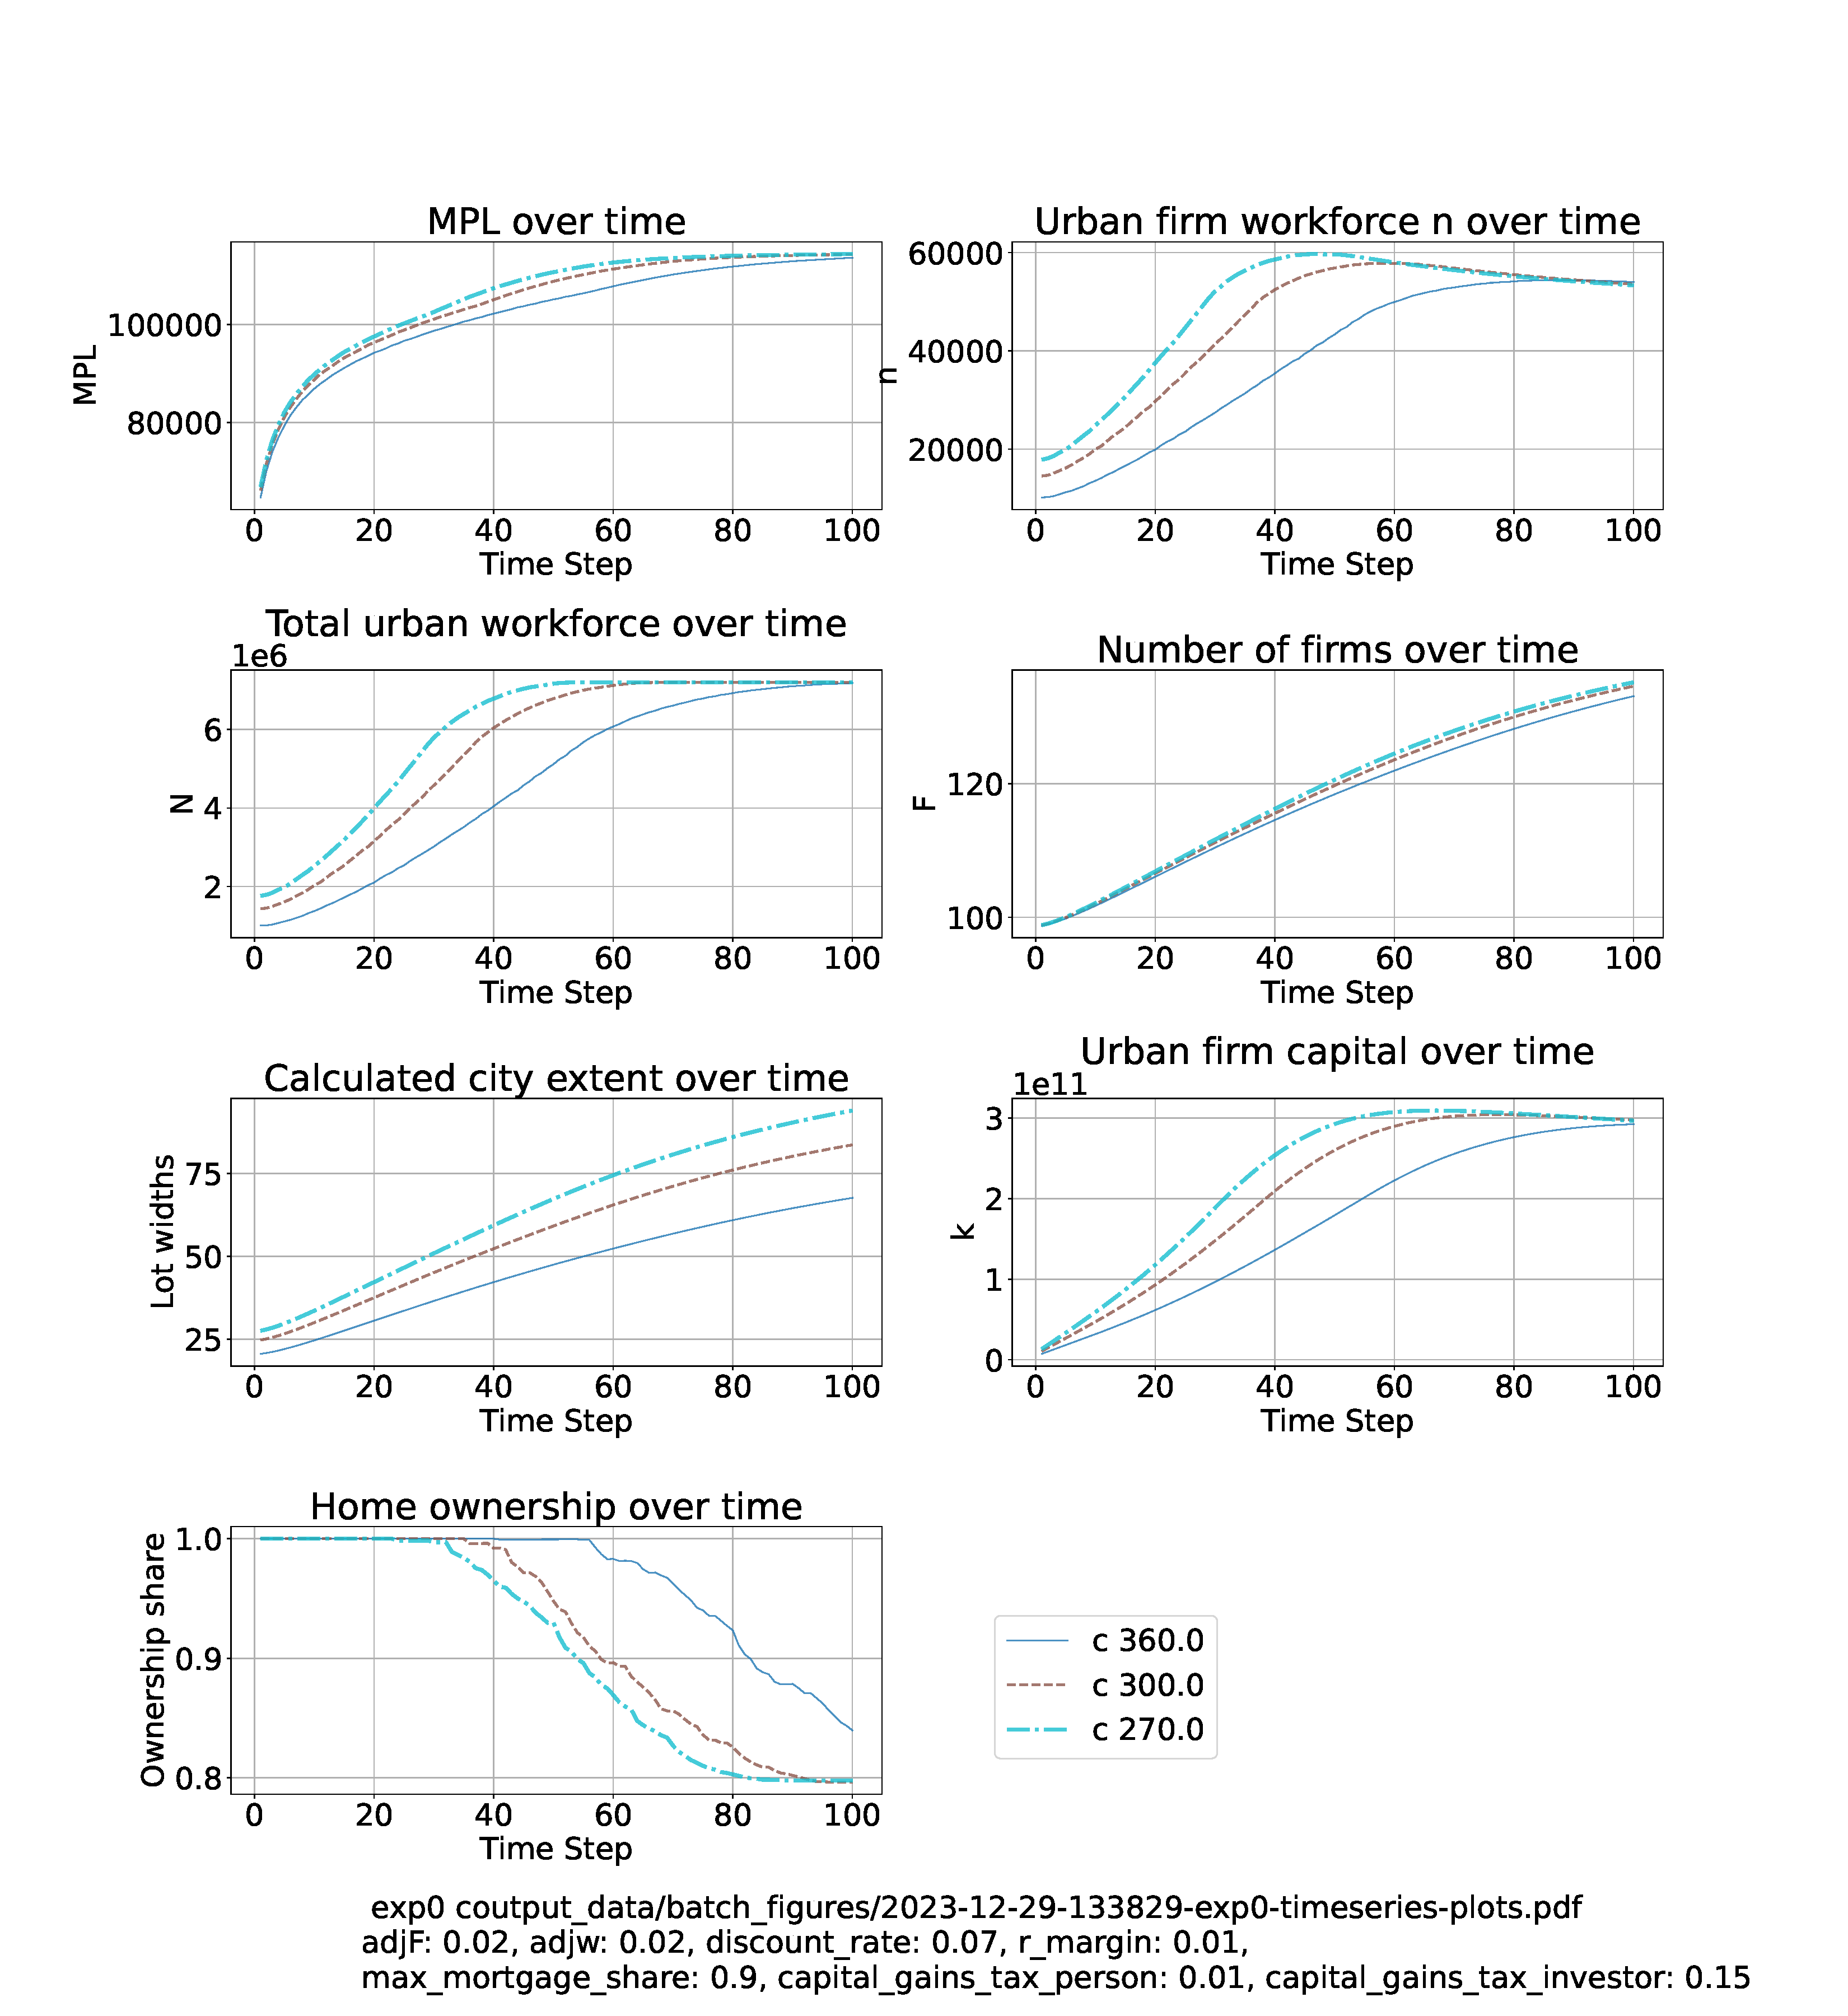
\includegraphics[trim= 1.5cm 3.65cm 2cm 4.0cm, clip, scale=.28]{fig/Analysis/Changing_Transport-cost2.pdf}

Transport cost affects both the total workforce and the total locational rents generated by a city. The response of the workforce is inversely proportional to the square of the transport cost.  

The figure above illustrates 10\% above and below our baseline value.  Reducing transport cost by 10\% increases population and total locational rents 10 \[\frac{1}{0.9 \times 0.9}=1.234568\]
the base value. This calculation assumes that wage and density do not respond as well but that the city extent does adjust.

\[Workforce\propto density * \pi \frac{\omega^2}{c^2}\]
\[Locational\ rents\propto density * \pi \frac{\omega^3}{c^2}\]\

\textbf{These relationships make transport costs the most influential single variable controlled by local authorities.} Transport systems, however, are costly in terms of land use and externalities generated or forgone.

The impact on housing ownership is curious. Home-ownership declines to about 



\newpage %%%%%%%%%%%%%%%%%%%%%%%%%%%%%%%%%%

\section{Capital gains tax for homeowners}
No noticeable sensitivity in any base outputs for this parameter. Ownership share exhibits at a tipping point at a personal capital gains tax rate of 0.25 when the capital gains rate for investors is 0.15. \textbf{(A gap is 0.1 in favour of households seems to be  needed to support homeownership.)}

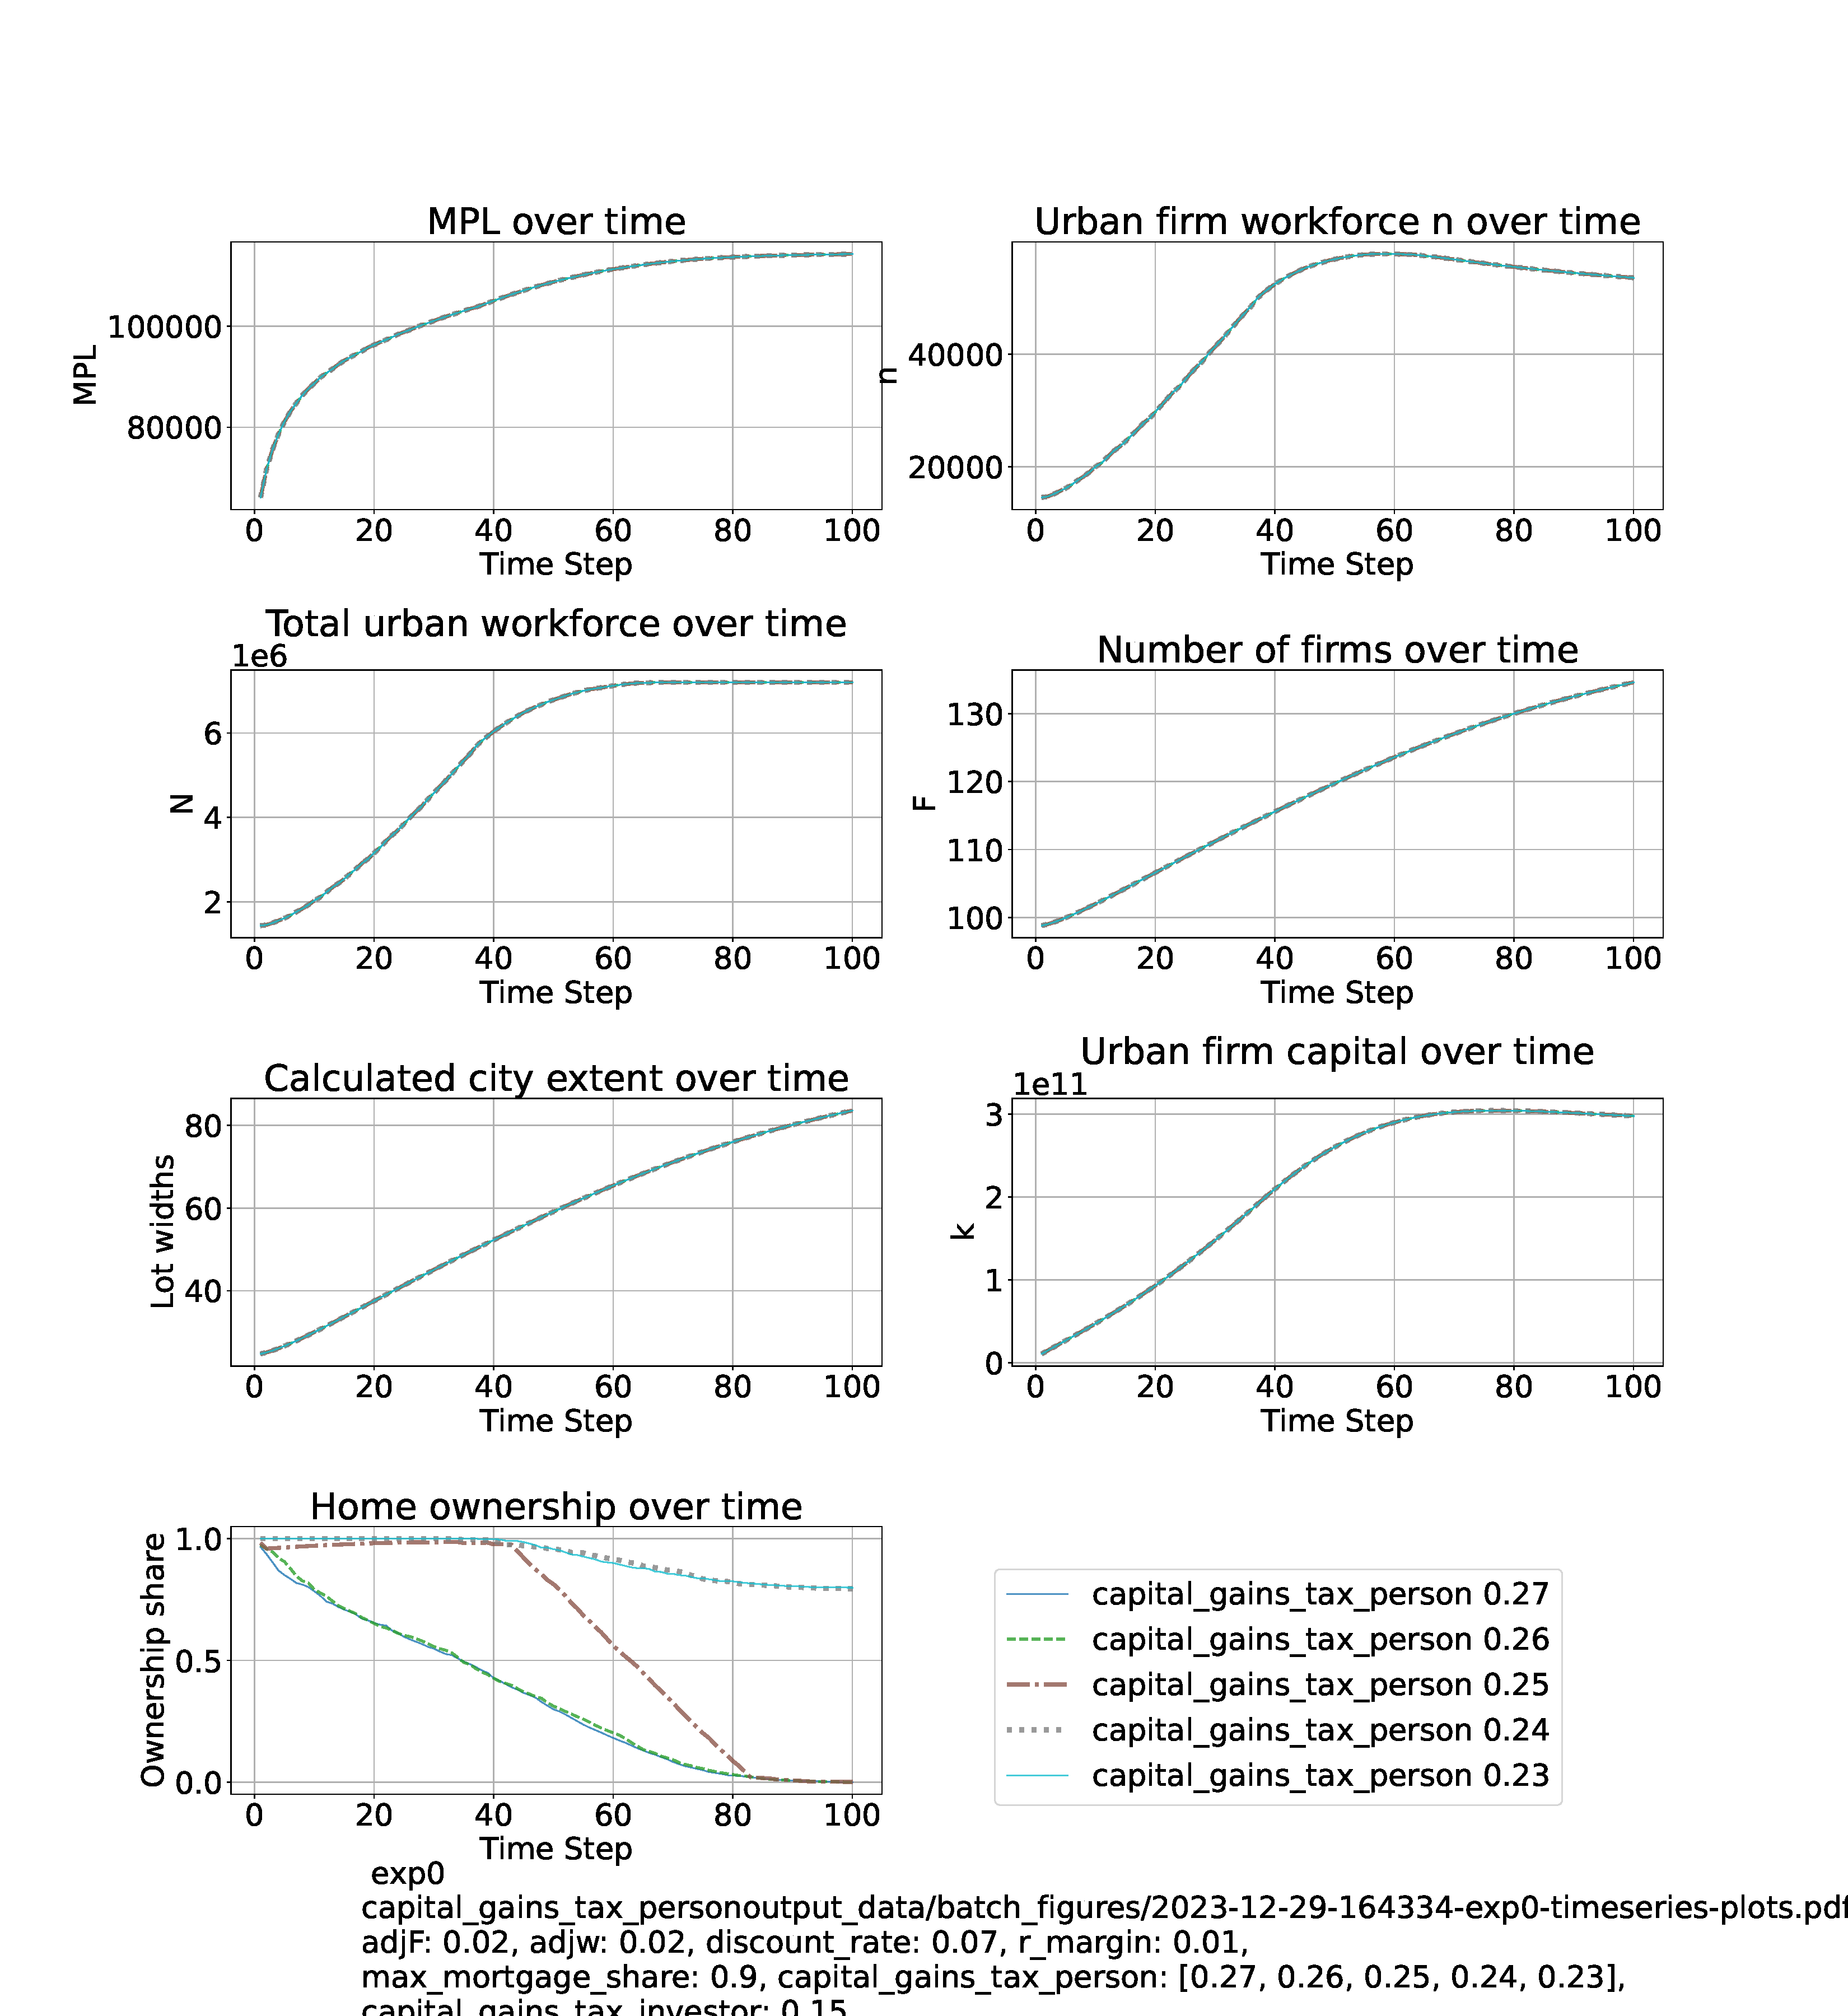
\includegraphics[trim= 1.5cm 3.65cm 2cm 4.0cm, clip, scale=.28]{fig/Analysis/Capital-gains-person-point27-6-5-4-3.pdf}



\newpage %%%%%%%%%%%%%%%%%%%%%%%%%%%%%%%%%%

\section{Capital gains tax for investors}
No noticeable sensitivity in any base outputs for this parameter.. Ownership share  exhibits at a tipping point at a personal capital gains tax rate of 0.25

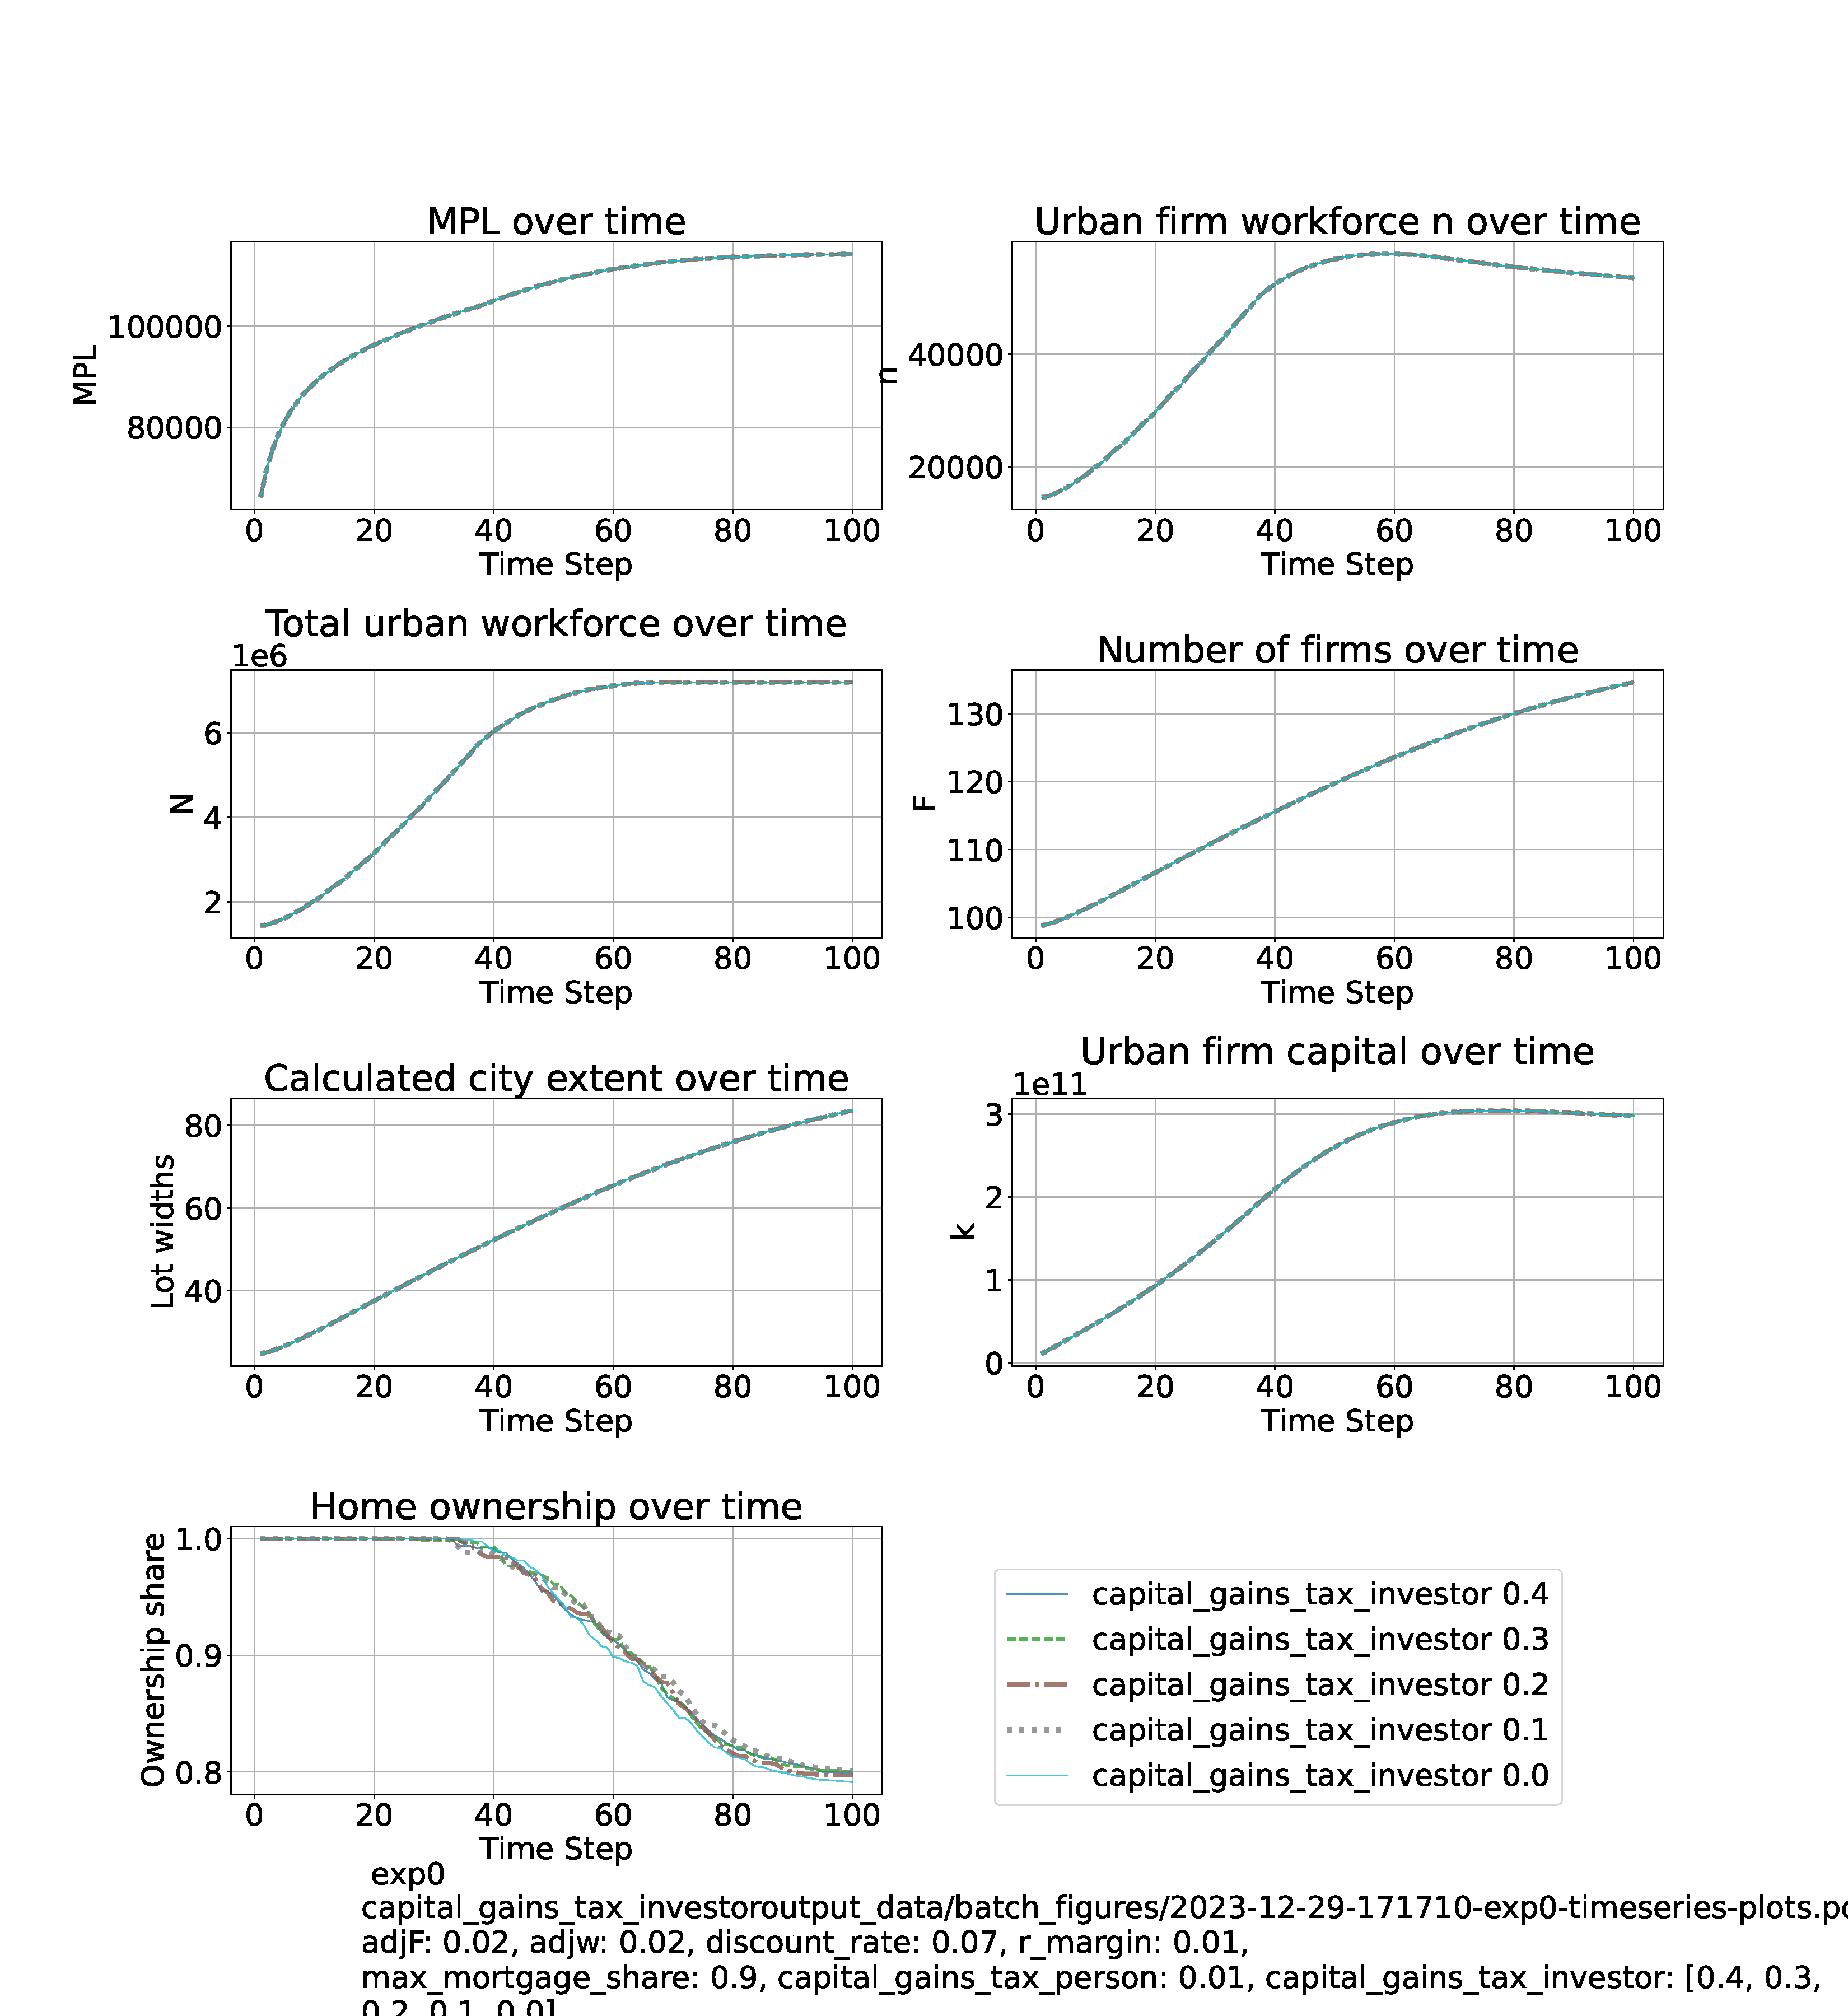
\includegraphics[trim= 1.5cm 3.65cm 2cm 4.0cm, clip, scale=.28]{fig/Analysis/Capital-gains-investor-point-4-3-2-1-0.pdf}



\newpage %%%%%%%%%%%%%%%%%%%%%%%%%%%%%%%%%%




\section{12-15 -010050 Change wealth sensitivity two cases 0.1 and 0.05 }
no sensitivity in any output for this parameter base. Ownership share may show  a small effect if we are near a tipping point driven by p-dot

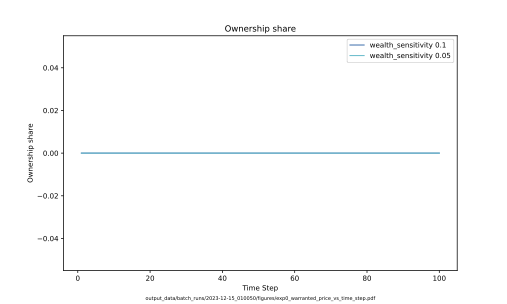
\includegraphics[scale=.45]{fig/Analysis/exp0_warranted_price_vs_time_step.png}


\begin{multicols}{2}
[\textbf{parameters}]
\begin{verbatim}
'adjn': 0.15,
'adjF': 0.02,
'adjw': 0.05, 
'capital_gains_tax_person':   0.0,
'capital_gains_tax_investor': 1,
\end{verbatim}

\end{multicols}
%%%%%%%%%%%%%%%%%%%%%%%%%%%%%%%%%%%%%%%%%%%%%
\newpage
\section{Change adjF - the growth rate of number of firms }

\begin{multicols}{2}
\begin{tabular}{c|c}
  mpl   &  up\\
  n   &  dn\\
  N   &  up\\
  F   & up \\
  E   &  up\\
  k   & dn
\end{tabular}

  notice the way firm number and size reverse as the adjustment speed changes. This makes sense
  
\end{multicols}

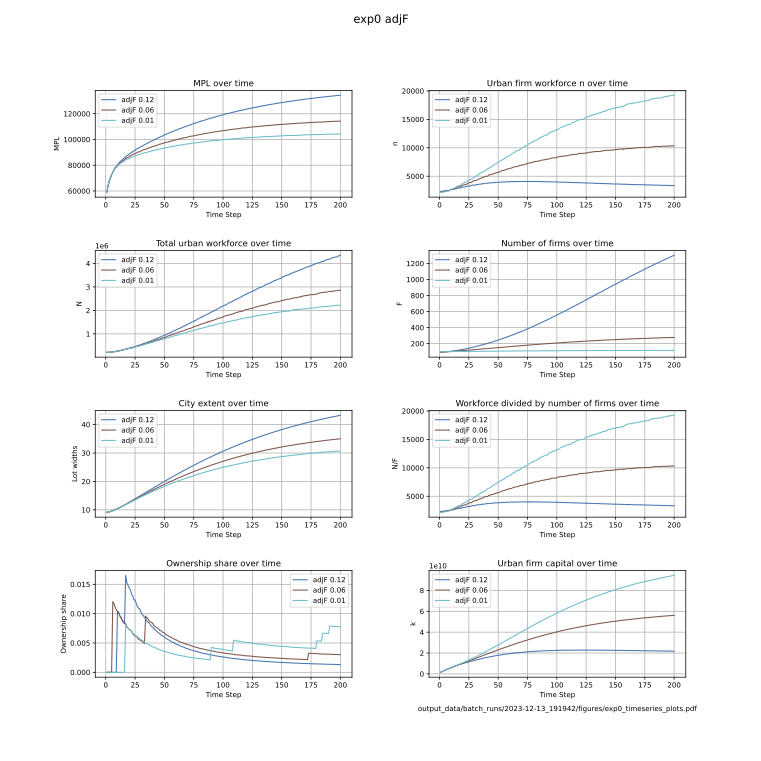
\includegraphics[scale=.55]{fig/Analysis/AdjF.png}

Notice too how MPL  is higher with a more rapid firm size adjustment. It keeps  firm workforce size down and pushes up MPL down, 

  Interestingly, city size is larger with faster growth of firm numbers. this is likely because with more firms hiring the population of the city grows faster.

%%%%%%%%%%%%%%%%%%%%%%%%%%%%%%%%%%%%%%%%%%%%%
\newpage
% \subsection{parameters}
% \begin{verbatim}

% \end{verbatim}

 \section{x12-15 010050, Change  Both adjF and adjn}
\begin{multicols}{2}
\begin{tabular}{c|c}
  mpl  &  \\
  n   &  \\
  N   &  \\
  F   &  \\
  E   &  \\
  k   & 
\end{tabular} 
Only three cases show (gold, turquoise, and purple). firm size and number show the same patternes as when just adF is changed 
\end{multicols}
% \begin{tabular}{l|c||c|c}
% parameters&&impact&\\ \hline
% & &  mpl  &  \\
% & &    n   &  \\
% & &    N   &  \\
% & & F   &  \\ 
% & &    Extent   &  \\
% & &    k   & 
% \end{tabular} 

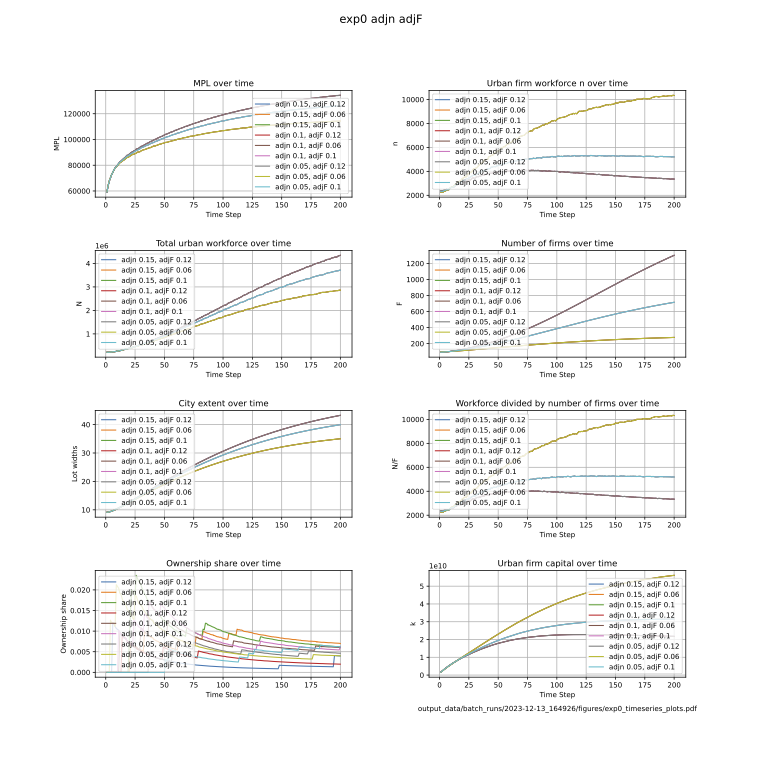
\includegraphics[scale=.55]{fig/Analysis/F-n-adjustment-speed.png}

% Subsistance wage typical 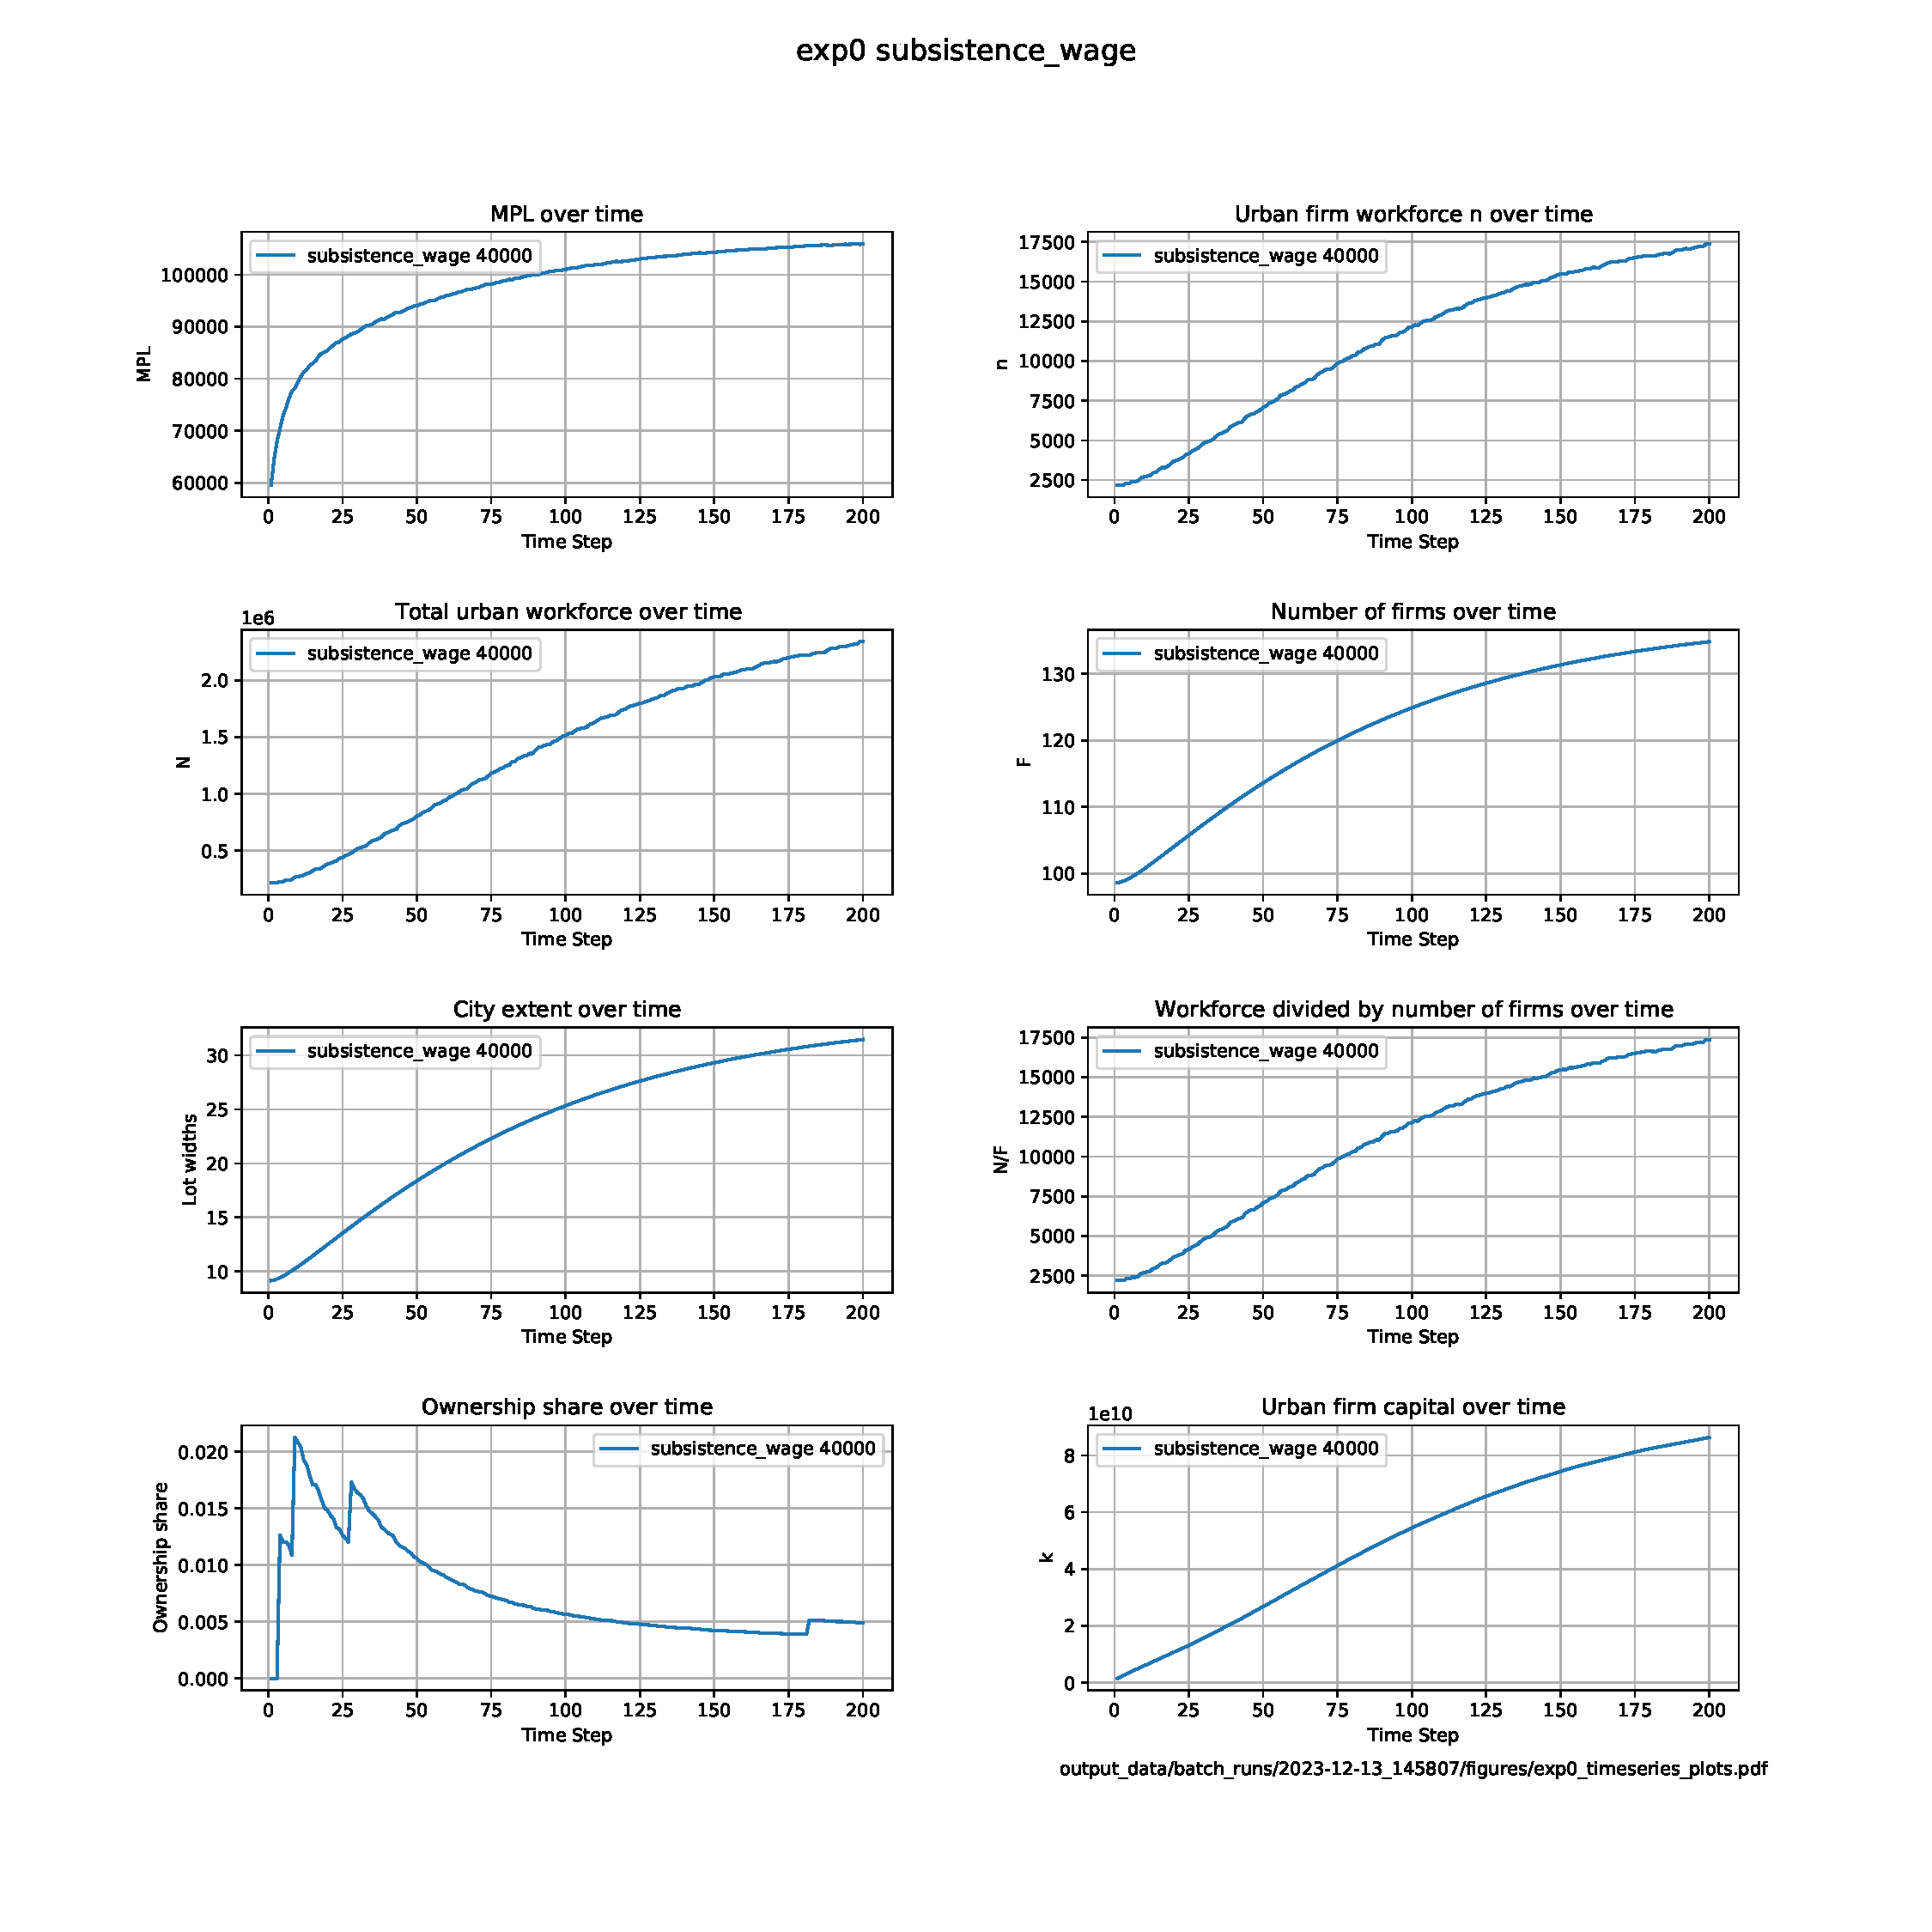
\includegraphics[scale=.55]{fig/Analysis/exp0-timeseries-plots.pdf}


We will want something like this perhaps in an early chapter. this case may not be interesting.
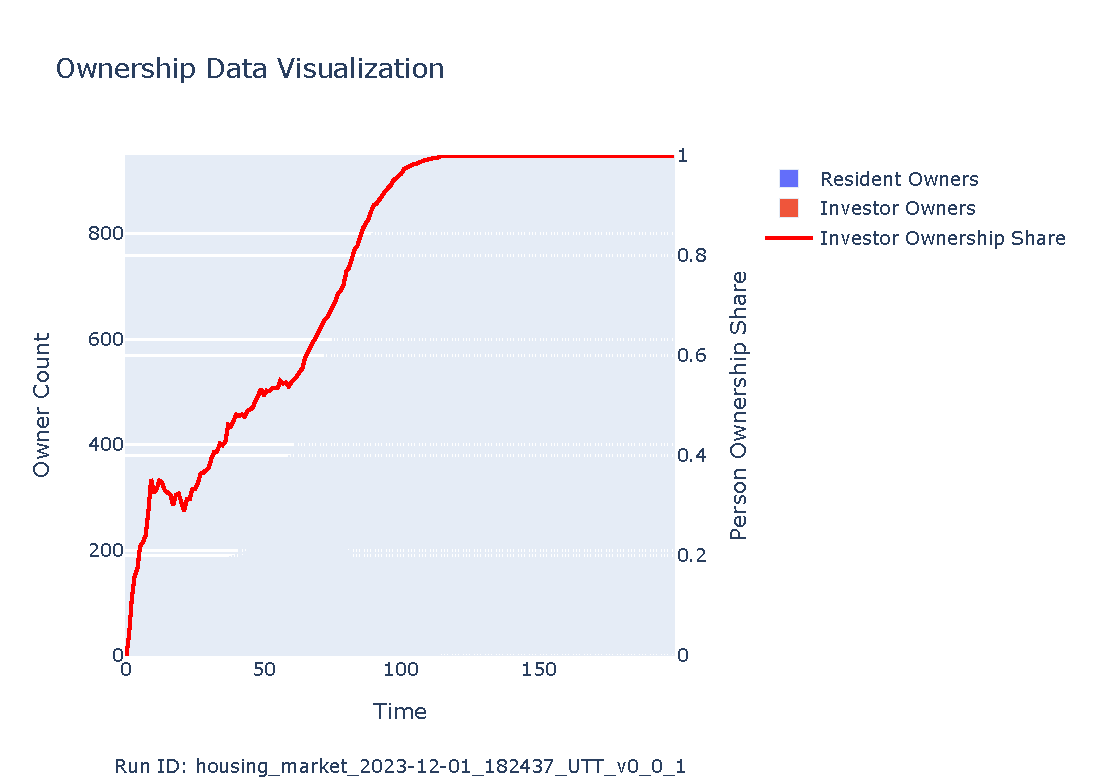
\includegraphics[scale=.95]{fig/Analysis/Ownership_Data_1.pdf}
% \subsection{parameters}
% \begin{verbatim}

% \end{verbatim}
\newpage
% \subsection{parameters}
% \begin{verbatim}

% \end{verbatim}

%%%%%%%%%%%%%%%%%%%%%%%%%%%%%%%%%%%%%%%%%%%%
 \section{12-17 010050, Varying Capital gains  }
\begin{tabular}{c|c}
  mpl  &  \\
  n   &  \\
  N   &  \\
  F   &  \\
  E   &  \\
  k   & 
\end{tabular} 

\includegraphics[trim= 1.5cm 5cm 2cm 6.5cm, clip, scale=.40]{fig/Analysis/215330-exp0-timeseries-plots.pdf}

% adjF: 0.02, adjw: 0.15, discount_rate: 0.07, r_margin: 0.01, max_mortgage_share: 0.9,  capital_gains_tax_person: [0.5, 0.01], capital_gains_tax_investor: [0.75, 0.5, 0.25

% \includegraphics[scale=.4, trim=2cm  5cm 2cm 4cm, clip]{fig/Analysis/2023-12-17_215330_exp0_timeseries_plots.pdf}

 \end{document}

 \newpage
% \section{parameters}
% \begin{verbatim}

% \end{verbatim}

% \section{Change  12-15 010050}
\begin{tabular}{c|c}
  mpl  &  \\
  n   &  \\
  N   &  \\
  F   &  \\
  E   &  \\
  k   & 
\end{tabular} 

 \includegraphics[scale=.25]{215330-exp0-timeseries-plots.pdf}
